\chapter{Teorie}
\label{2-Teorie}

\section{OpenStreetMap}
\label{OpenStreetMap}

\subsection{Vznik}
\label{vznik}
OpenStreetMap (OSM) je projekt, jež vznikl s cílem vytvoření a sběru 
volně dostupných geografických dat a následně jejich možné vizualizace
do topografických map. Projekt založil Steve Coast v červenci roku 
2004 v Anglii. Jako inspirace mu posloužil projekt Wikipedia.

Zprvu projekt využívalo jen pár nadšenců, postupem času ale získal
%%% ML: dvakrat "narustat" v jedne vete
projekt popularitu. S nárůstem počtu uživatelů narůstal i objem dat.
%%% ML: nejen kapacitu serveru, ale cele infrastruktury, resit dalsi otazky (bezpecnost a pod)...
Bylo tedy nutné zvyšovat kapacitu serverů. 

V dubnu roku 2006 byla založena nadace OpenStreetMap Foundantion pro financováni 
projektu jako takového (zaměstnanců, běhu serverů atd.). \cite{wikiOSM}


\subsection{Struktura dat}
\label{struktura dat}
OSM data jsou nyní ukládána v databázi PostgreSQL \footnote{viz \url{http://blog.cleverelephant.ca/2009/04/openstreetmap-moves-to-postgresql.html}}
%%% ML: tady to skoro vypada, ze jsou dava ve formatu XML ulozena
%%% primo v DB, cemuz tak ale neni; XML, resp. OSM je vymenny format
a jsou k dispozici ve formátu XML. Jeho výhoda je jasná 
struktura, snadná orientace v kódu pro člověka. Nevýhodou je ovšem větší objem
%%% ML: v jake slova smyslu (prvek ~ soubor) ???
dat, který lze ale snížit kompresí. Každý prvek má vlastní XML soubor. 

%%% ML: tady by se hodil vycet (itemize), chtelo by do vysvetlit, co je cesta a pod...
Třídy prvků v OSM jsou rozděleny na: uzel (node), cesta (way) a
relace (relation).

Příklad XML souboru pro cestu:

{\scriptsize
\begin{lstlisting}
<osm version="0.6" 
generator="CGImap 0.4.0 (32632 thorn-01.openstreetmap.org)" copyright="OpenStreetMap and contributors" attribution="http://www.openstreetmap.org/copyright" license="http://opendatacommons.org/licenses/odbl/1-0/">
   <way id="87249754" visible="true" version="2" changeset="34489106" timestamp="2015-10-07T11:52:41Z" user="Petr Dlouhý" uid="17615">
       <nd ref="1014526199"/>
       <nd ref="1014525941"/>
       <nd ref="1014526337"/>
       <nd ref="1014526022"/>
       <nd ref="1014526277"/>
       <nd ref="1014525984"/>
       <tag k="highway" v="path"/>
       <tag k="source" v="bing:ortofoto"/>
   </way>
</osm>
\end{lstlisting}
}


Uzel je definován jedinečným identifikátorem ({\tt node id=}). Jeho
%%% ML: dodat EPSG kod, vsechny souradnice jsou v jednom SRS...
souřadnice jsou ve WGS~84. Je také ukládána verze ({\tt version= }) a kdy
%%% ML: opet cestina (minimalne 2x "a")... preformulovat
byl do databáze přidán a v jaké změně to bylo provedeno ({\tt changeset=~}).
%%% ML: cely tento odstavec plati i pro dalsi elementy - way/area (?)
Dále k bodu je možné připojit různé atributy s klíčem a hodnotou ({\tt tag~k=~v=~}).

Linie je spojení dvou a více uzlů, dále má také svůj identifikátor ({\tt way~id=~}).
%%% ML: nejde o hlavicku, ale o xml atributy a tagy...
Hlavičku XML souboru má shodnou s bodem. Ale dále obsahuje také seznam id uzlů,
které ji tvoří. Liniím lze taktéž přiřadit atributy.

Linie lze ještě rozdělit na neuzavřené a uzavřené. Uzaveným liniím lze připojit
i atributy určené jen pro plochy. Například les ({\tt landuse=forest}).
%%% ML: veta nize - ?
V případě, když se přidá atribut, který je prot linie, ale chceme
ho použít pro plochy, musí se ještě přidat se atribut {\tt area=yes}.

Speciálním příkladem jsou relace ({\tt relation= }), do kterých lze zahrnout
jeden a více prvků. Lze do nich spojit prvky stejné, nebo odlišné třídy,
nebo i jiné relace. Například dálnice je tvořena několika liniemi (cestami), a ty
jsou zahrnuty do společné relace Dálnice D1. Nebo např. turistická trasa
(od~KČT) je relace sdružující jak linie (cesty, pěšiny) tak i uzly
(rozcestníky, vyhlídky, apod. ).

%%% ML: osm wiki zni familiarne, + reference v tomto pripade je lepsi
%%% hned za slovem, nemusim byt na konco odstravce
U atributů popsaných na osmwiki \cite{OSMfeatures} je vždy uvedeno, k jaké třídě je
vhodné a nevhodné je použít (dle komunity uživatelů OSM). Pokud se stane, že je použit
%%% ML: to ???
na~jinou než povolenou třídu, nemusí to hlásit chybu, ale může být následně
%%% ML: viz kapitola?
problém v některých vykreslovačích. 

\subsection{Změna licence}
\label{změna licence}

%%% ML: Původně vs. původní data...
Původní data OSM a generované grafické dlaždice
byly na distribuovány pod licencí
Creative~Commons~AllributionShare~Alike 2.0 (CC~BY~SA~2.0).

Tato licence umožňovala užití (distribuci ale i editaci) díla pod podmínkou,
že bude uveden zdroj OpenStreetMap.org ve viditelné části
vytvořených mapových dlaždic \cite{OSMlicence}.

  \begin{figure}[hbt]
    \centering
      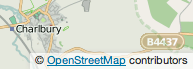
\includegraphics{./pictures/attribution_example.png}
      \caption{Příklad umístění licence}
      \label{fig:attribution_example}
  \end{figure} 

%%% ML: duvod zmeny ?
V roce 2012 byla licence publikovaných dat změněna na Open Data Commons
Open Database Licence (ODbL).
Tato změna licence přinesla problém
s~daty, které byly poskytnuty projektu v předchozí licencí
(CC~BY~SA~2.0). Bylo nutné se dotázat každého z dřívějších
přispěvatelů dat, ať už právnických osob, tak i fyzických osob, jestli
%%% ML: slo o to, zda souhlasi aby jejich prispevky byly poskytovany
%%% pod novou licenci, veta to naznacuje, ale je nepresna
s touto změnou souhlasí a je možné s jejich daty i s novou licencí
nakládat. U přispěvatelů, kteří nedovolili užívání jejich díla
%%% ML: co vymazat - jejich prispevky - preformulovat
pod novou licencí, nebo u těch, co se nevyjádřili, bylo nutné
%%% ML: chybi reference, co znamena zlomek?
z~databáze vymazat. Tato situace nastala pouze ve zlomku případů.
%%% ML: v jake mire? doplnit
Nejvíce tato změna licencí ohrozila data v zemích jako je Polsko a Nový Zéland.

%%% ML: proc tento dualismus?
V současnosti jsou tedy data OSM distibuována pod licencí ODbL a
generované grafické dlaždice pod licencí CC-BY SA 4.0
\cite {OSMlicenceIssue}.

\subsection{Licence ODbL}

%%% ML: preformulovat: Licence ODbl umoznuje...
Ve zkratce s daty pod licencí ODbL uživatel smí:
\begin{itemize}
    \item    kopírovat, distribuovat a užívat data
    \item    vytvářet nová data z původních
    \item    měnit původní data
\end{itemize}

%%% ML: preformulovat
S použitím ale uživatel musí ale uvést zdroj a licenci dat.
Dále uživatel souhlasí, že nová data vytvořená z původních dat budou sířena
také pod~licencí ODbL.
Podrobněji viz přesné znění licence na stránkách OpenDatabase.\footnote{http://opendatacommons.org/licenses/odbl/1.0/}


\subsection{Zdroje dat}
\label{Zdroje dat}

Jak bylo zmíněno, byla snaha, aby mapová data tvořili jedinci vlastním
sběrem dat. Sběr dat ve smyslu měřením vlastní GNSS (GPS, Glonass)
přijímačem a znalost místních poměrů (uzavřené silnice, stezky atd.).
Toto mapové dílo z těchto dat mohli volně užívat k vlastním užití.
Komunita přispěvatelů se zprvu pomalu, ale později rychle rozrostla a
dnes čítá 3,7 milionů registrovaných uživatelů s alespoň jednou
vytvořenou změnou v OSM a 2,7 milionů účtů aktivních přispěvatelů.\cite{OSMstats}

Tyto mapové podklady byly velice vhodné i pro další projekt, dnes již
velice rozšířený a známý jako Geocashing (GC). Projekt GC začal mapové
podklady od OSM užívat a zároveň jeho uživatelé začali sami tvořit a
přispívat do OSM. 

Přispěvatelé dat do OSM musí respektovat, že OSM je pod licencí OdbL.
Tudíž i jejich zdroj dat musí splňovat tuto licenci. Proto by měli
všechny svoje změny, které v OSM vytvoří, řádně ozdrojovat atributem
s~klíčem 
{\tt source= }
V případě vlastního sběru dat se vyplňuje hodnotou
{\tt source=survey} ,
popřípadně uvést zdroj, odkud čerpali. Pokud tuto povinnost poruší a
použijí zdroj, jež není kompatibilní z politikou OSM, tak samotné OSM
jejich změnu, aby předešel sporům, sám vymaže. Bohužel musí vymazat
celou sadu změn, byť by v něm byl jeden prvek, jenž toto poruší.

Druhým významným zdrojem dat jsou soukromé subjekty (společnosti) a
většinou jde o podkladové zdroje dat, například ortofoto. Pro obkreslování
silničních síti z~leteckých nebo satelitních rastrů. V~jejich případě to
bylo řešeno písemným svolením, nebo smlouvou. Jako významným zdrojem byla
společnost Bing, jež nabídla k~dispozici letecké snímky většiny
obydlené pevniny. 

Třetím zdrojem a zároveň postupně dominujícím, co do obsahu dat, jsou
databáze ze státního sektoru. Tyto databáze jsou nejvhodnějším zdrojem
dat.

\subsection{Vykreslovače}
\label{Vykreslovače}
Na hlavní stránce OSM je pět „základních“ přednastavených vrstev vykreslených 
z~dat z OSM. Využívá aplikaci OpenLayers založenou na konceptu AJAX.
Pro snadné vykreslení dat do grafických dlaždic se používá Mercatorovo zobrazení.

\begin{itemize}

  \item Standardní vrstva - vykresluje všechny prvky přiměřeně.
  \item Cyklomapa - vykresluje cyklostezky, výškopis. 
  \item Dopravní mapa - vykresluje silniční a železniční sítě.
  \item MapQuest Open vznikla jako podkladová mapa právě pro potřeby 
Geocaching.
  \item Humanitární mapa, která vykresluje služby (restaurace, banky, muzea, 
  školy, kostely...)  a potlačuje ostatní prvky. 

\end{itemize}

Existují další stránky, jež se zabývají vlastní kompozicí a vykreslením
různých dat. Například mapu turistických a cyklistických tras vykresluje
pro celou Evropu mtbmap.\footnote{mtbmap.cz}

Zajímavými projekty jsou například ty, které k 2D mapě přidávájí „třetí“ rozměr a
vytvářejí tzv. 2.5D mapu. Většinou jde o 3D zobrazení budov, mostů (dle
atributů), popřípadě i stromů.

\section{Opendata}
\label{opendata}
Základní myšlenka otevřených dat vznikla v USA z iniciativy vlády Barracka Obamy.
Tedy pokud vzniknou geografická data z veřejných peněz, měla by tedy být
přístupná veřejně. Mělo to kladný efekt na tamní ekonomiku. Díky tomuto byly
zprvu k~dispozici satelitní snímky povrchu Země a digitální model terénu
s~rozlišením 30x30 m od NASA (pro pozdější vykreslení vrstevnic).

Tento trend se začal rozšiřovat zprvu do zemí západní Evropy,
jmenovitě Anglie, Francie, ale i jiné země mimo Evropu..

V ČR se tomuto věnuje fond Otevřená data\footnote{www.otevrenadata.cz}, který založil Otakar
Motejl. Tento fond spolupracuje s nadací Sociery Fund Praha. V rámci
těchto uskupení je vyvíjen tlak na transparentnost veřejné správy a
zveřejňování smluv a dat
státních institucí, jelikož jejich získání a údržba byla placena
z~veřejných zdrojů.



\section{Importy}
\label{Importy}
Výraz import v tomto případě znamená začlenění většího množství datových sad
z~jednoho datového úložiště (databáze serveru) na jiný. Při velkých objemech dat
se využívá výkonu výpočetní techniky z důvodu její bezchybovosti, a také
z~důvodu časové náročnosti. Na člověku poté ale zbývá zvolit postup importu
a naprogramovat skript nebo program, podle něhož technika samotný proces
provede. 

Datové importy z veřejných databází do databáze OSM jsou velmi cenné. 
Otevřené geografické, ale i jiné, databáze státu a jeho veřejných institucí 
financovaných státem jsou komplexní. Komplexní v tom smyslu, že obsahují celistvý
soubor dat, protože je daná instituce vyžaduje ke svém chodu. Jistá nevýhoda tu 
ale může být, a to, že data nemusí být vždy úplně aktuální. Některá data mohou 
být sbírána a zveřejněna i s větším časovým odstupem.

V rámci České Republiky proběhlo již několik hromadných datových importů. Jak 
již bylo řečeno, větší časová náročnost zabere samotná příprava na import. A to
v~případě, importu do OSM. Nejen napsání skriptu, ale i nutná diskuze tohoto záměru
na~diskuzní konferenci Talk-cz. 

\subsection{Talk-cz}
\label{Talk-cz}
Tato diskuze probíhá přes posílání emailových zpráv do společné konference. 
Uživatelům chodí emaily z probíhající diskuze a pokud na nějaký chtějí reagovat,
tak pošlou email na adresu serveru, na kterém diskuze běží, a musí do Předmětu 
napsat Re: a předmět zprávy, na kterou reagují. Server tyto zprávy pomocí 
předmětu a času řadí. Diskuze je poté k dispozici na webových stránkách.\footnote{http://lists.openstreetmap.org/listinfo/talk-cz}

\section{IPR Praha}
\label{IPR Praha}
IPR Praha je zkratka názvu Institut plánování a rozvoje a hlavního města Prahy. 
Tento institut se věnuje urbanismu, architektury a rozvoje města Prahy. Hlavním
úkolem IPR je tvorba územního plánu Prahy a významným úkolem IPR je zajišťovat
zpracování geografických informací. Spravuje data a mapy města Prahy. Od roku 
2002 poskytuje na svých stránkách zdarma webové aplikace bez limitu využití. 
Po~rozvoji Pražského geoportálu došlo k jejich většímu využívání.  Na základě 
platných Pravidel pro poskytování dat a  výstupů z datových souborů a datového 
skladu Geografického byla od dne 1.~4.~2015 zveřejněny datové soubory a další 
webové služby. Tato data byla uveřejněna pod licencí CC-BY SA 4.0 \cite{IPR}
\subsection{licence CC BY-SA 4.0}
\label{licence CC BY-SA 4.0}
Licence CC BY-SA 4.0 je zde uvedena ve zjednodušeném znění.

"Uživatel s smí
\begin{itemize}
    \item   Sdílet - rozmnožovat a distribuovat materiál prostřednictvím jakéhokoli média v jakémkoli formátu
    \item   Upravovat - remixovat, změnit a vyjít z původního díla
\end{itemize}
pro jakýkoliv účel, a to i komerční.

Poskytovatel licence nemůže odvolat tato oprávnění do té doby, dokud dodržujete licenční podmínky.

Uveďte původ — Je Vaší povinností uvést autorství, poskytnout s dílem odkaz na licenci a vyznačit Vámi provedené změny. Toho můžete docílit jakýmkoli rozumným způsobem, nicméně nikdy ne způsobem naznačujícím, že by poskytovatel licence schvaloval nebo podporoval Vás nebo Váš způsob užití díla.

Zachovejte licenci — Pokud budete toto dílo upravovat, pozměňovat nebo na něj navazovat, musíte svoje odvozená díla vystavovat pod stejnou licencí jako původní dílo."

Podrobněji viz přesné znění na stránkách CraetiveCommmons.
\footnote{https://creativecommons.org/licenses/by-sa/4.0/legalcode/}


\section{PostgreSQL}
\label{PostgreSQL}
PostgreSQL je Opensource databázový systém, který je vyvýjen déle než patnáct
let. Za dlouhou dobu vývoje se stal robustní a také hojně využívaný.
Postupem času získal svou spolehlivostní silnou reputaci.
Lze s ním pracovat ve všech známých operačních systémech. 
...
\cite{PostgreSQL}

\subsection{PostGIS}
\label{PostGIS}
PostGIS je objektově-relační nadstavba databázové struktury PostgreSQL.
Rozšiřuje ji o funkce, které umožňují geometrické operace s objekty v ní uložené.
Třídy prvků mohou být buď bod (point), linie (line) nebo polygon (polygon).
Dále je možné více prvků jedné třídy sdružit do multi-relace, 
to jest  multiPoint, multiLine, multiPolygon.
Geometrie prvku určuje jeho polohu v určité souřadnicové soustave, neboli 
kartografickém souřadnice. Dále určuje i kartografickou soustavu, ve které je 
jeho geometrie určena. Je tedy dále možné při známých transformacích mezi
soustavami provádět transformace souřadnic. Základní operace jako délka, obvod,
plocha, ale jsou zde i sofistikovanější funkce, které lze s objekty nebo i mezi 
objekty provádět.

Sotware PostGIS je šířen pod GNU General Public License (GPLv2) licencí.


\section{Python}
\label{Python}
Programovací jazyk Python vznikl v roce 1991. Navrhlo ho Guido van Rossum. 
Je vyvíjen jako open source projekt. Inspiroval se hlavně programovacím jazykem
ABS, který byl přímo vytvořen pro~výuku začatečníků v programování. Python je 
proto jeden z nejvýhodnějších programovacích jazyků pro začínající programátory,
ale i přesto ho lze použít pro~praktické programování. 

Jedná se tedy o jednoduchý programovací jazyk podporující různá programovací 
paradigmata, hlavně objektové, imperiativní, procedurální a omezené míře i 
fun- kcionální. Je multiplatformní, lze jej tedy použít na různých operačních 
systémech. Klade velký důraz na syntaxi psaného kódu, využívá hlavně prázdné 
znaky v~psaném kódu.  

Programy nebo skripty lze psát v textovém editoru, ale je vhodné použít 
standartu PEP~8, který kontroluje prázdné znaky a správnou strukturu skriptu. 

V současné době je vydána stabilní verze 3.5.7, která vůči předchozí verzi 2.x
mění některá, již "zažitá" syntaxe. Například nejviditelnější je změna funkce 
{\tt print } pro verzi 2.x stačilo  {\tt print 'Ahoj'}  a pro verzi 3.x je již
nutné string vložit do závorek  {\tt print('Ahoj')}  . Tyto dvě dnes používané
verze 2.x a 3.x jsou navzájem nekompatibilní.
\cite{python} 
\cite{wikiPython} 
  
  
\subsection{knihovna argparse}
\label{argparse} 
Knihovna argparse, jejíž autor je Tshepang Lekhonkhobe, je knihovna 
do~programovacícho jazyku Pyhon. Řeší konzolový vstup do aplikace a zpracovává 
ho pro další použití v programu.\cite{argparse}


\subsection{knihovna xmltodict}
\label{xmltodict} 
Tato knihovna umí číst soubory ve formátu XML a zpracovává je do snažší formy 
dat, která je jednodušší manipulaci pro samotný program. Data z XML zpracuje
do formy datové řady (array), kde každý člen této řady může být opět řada dat.\cite{xmltodict}

příklad parsování dat ve XML formátu

{\scriptsize
\begin{lstlisting}
<head>
  <many>ele1</many>
  <many>ele2</many>
</head>
\end{lstlisting}
}

Po otevření a parsování se v Python(u) provede příkazem.

{\scriptsize
\lstset{language=Python}
\begin{lstlisting}
with open('example.xml') as fd: 
  doc = xmltodict.parse(fd.read()) 
\end{lstlisting}
}

Objekt {\tt doc} má poté podobu.

{\scriptsize
\lstset{language=Python}
\begin{lstlisting}
OrderedDict([(u'head', OrderedDict([(u'many', [u'ele1', u'ele2'])]))]) }
\end{lstlisting}
}

V této datové řadě lze již snadno procházet. 

{\scriptsize
\lstset{language=Python}
\begin{lstlisting}
doc['head']['many'][0]
ele1
\end{lstlisting}
}


\subsection{knihovna GDAL/OGR}
\label{GDAL/OGR}
Jedná se o knihovnu pro práci s geografickými daty a umožňuje jejich čtení a zápis.
Je psána v programovacím jazyce C++. Je považován za jeden z hlavních 
open~source projektů a je hojně používán ve sféře GIS. Pracuje s vektorovými a 
rastrovými datovými formáty. Podporuje velkou škálu souborových formátů, a to 
pro vektorová data, ale i pro rastrová. Obsahuje databázi definic kartografických
projekcí používaných na celém světě a databázi jejich známých transformací. 
Umožňuje tedy komplexní operace s geografickými daty. \cite{GDAL}


\section{QGIS}
\label{QGIS}
QGIS je program vytvořen za účelem prohlížení a editace geografických dat.
Jedná se o Opensource software. Je tedy možné, aby na jeho vývoji spolupracoval
kdokoli. Je možné si vytvářit novou funkci, nebo přímo zásuvný modul do programu.
Je možné je psát v jazyce C++ nebo Python.
Tyto moduly si uživatelé mohou poté stáhnout a přidat do QGISu a využívat.
QGIS také umožňuje využívat konzolově jazyk Python. Je možné si tak vytvářet
vlastní jednoduché skripty v jazyce Python a spouštět je v QGISu.

Od svého vzniku bylo vydáno již spoustu verzí programu.
Dříve byly verze pojmenovávány podle planet, později podle jejich měsíců a nyní se dávají
jména německých měst. V současnosti (duben 2016) je k dispozici verze 2.14 Essen
